\section{Hearst Patterns}
\label{sec:hearst-patterns}

\begin{frame}
  \frametitle{Hearst Patterns}

  \makebox[\textwidth][c]{
    \begin{tikzpicture}
      \node[align=center, rectangle] at (0, 3.5) {Hypernym};
      \node[align=center, rectangle] at (6, 3.5) {Hyponym};

      \node[align=center, rectangle] (A) at (0, 0) {car \\ color};
      \node[align=center, rectangle] (B) at (6, 1.6) {BMW \\  Mercedes
        \\ Audi};
      \node[align=center, rectangle] (C) at (6, -1.6) {red \\ gray \\ blue
        \\ black};


      \node[draw, fit=(A), circle, scale=1.5] {};
      \node[draw, fit=(B), circle, scale=1] {};
      \node[draw, fit=(C), circle, scale=1.025] {};

      \draw [->] (0.35, 0.25) -- (4.65, 1.5);
      \draw [->] (0.35, -0.25) -- (4.65, -1.5);
    \end{tikzpicture}
  }
\end{frame}

\begin{frame}
  \frametitle{Hearst Patterns: Regelen}

  $$R \subseteq M \times M$$
  $$\forall x, y, z \in M : xRy \land yRz \Rightarrow xRz$$
  $$\forall x \in M : \neg xRx$$
  $$\forall x, y \in M : xRy \Rightarrow \neg (yRx)$$
\end{frame}

\begin{frame}
  \frametitle{Hearst Patterns: Definitionen}

  \begin{itemize}
  \item $NP_{X} \rightarrow Hypernym$
  \item $NP_{Y} \rightarrow Hyponym$
  \end{itemize}

  \begin{itemize}
  \item $NP_{X}$ and other $NP_{Y}$
  \item $NP_{X}$ or other $NP_{Y}$
  \item $NP_{Y}$ such as $NP_{X}$
  \item Such $NP_{Y}$ as $NP_{X}$
  \item $NP_{Y}$ including $NP_{X}$
  \item $NP_{Y}$, especially $NP_{X}$
  \item $NP_{Y}$ like $NP_{X}$
  \end{itemize}
\end{frame}

\begin{frame}
  \frametitle{Hearst Patterns: Regulärer Ausdruck}

  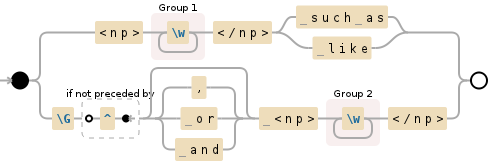
\includegraphics[scale=0.63]{img/regex}
\end{frame}